% ============================================================================
% NEURAL SEARCH: ICLR-LEVEL WHITEPAPER
% A comprehensive scientific and mathematical foundation
% ============================================================================
\documentclass{article}

% ICLR 2024 style formatting
\usepackage[utf8]{inputenc}
\usepackage[T1]{fontenc}
\usepackage{hyperref}
\usepackage{url}
\usepackage{booktabs}
\usepackage{amsfonts}
\usepackage{nicefrac}
\usepackage{microtype}
\usepackage{xcolor}
\usepackage{amsmath,amssymb,amsthm}
\usepackage{mathtools}
\usepackage{algorithm}
\usepackage{algpseudocode}
\usepackage{graphicx}
\usepackage{subcaption}
\usepackage{tikz}
\usetikzlibrary{arrows.meta,shapes,positioning,calc,fit,backgrounds,decorations.pathmorphing,patterns}
\usepackage{pgfplots}
\pgfplotsset{compat=1.17}
\usepackage{multirow}
\usepackage{tabularx}
\usepackage{enumitem}
\usepackage{natbib}
\usepackage{float}
\usepackage{wrapfig}

% Page geometry - conference style
\usepackage[margin=1in]{geometry}

% ============================================================================
% THEOREM ENVIRONMENTS
% ============================================================================
\theoremstyle{definition}
\newtheorem{definition}{Definition}[section]
\newtheorem{theorem}{Theorem}[section]
\newtheorem{lemma}[theorem]{Lemma}
\newtheorem{proposition}[theorem]{Proposition}
\newtheorem{corollary}[theorem]{Corollary}
\newtheorem{remark}{Remark}[section]
\newtheorem{example}{Example}[section]

% ============================================================================
% CUSTOM COMMANDS
% ============================================================================
\newcommand{\dataset}{\mathcal{D}}
\newcommand{\query}{\mathbf{q}}
\newcommand{\score}{\text{score}}
\newcommand{\embed}{\phi}
\newcommand{\graph}{\mathcal{G}}
\newcommand{\nodes}{\mathcal{V}}
\newcommand{\edges}{\mathcal{E}}
\newcommand{\rel}{\text{rel}}
\newcommand{\confidence}{\gamma}
\newcommand{\evidence}{\mathcal{E}}
\newcommand{\fingerprint}{\mathbf{f}}
\newcommand{\compatibility}{\kappa}
\newcommand{\RRF}{\text{RRF}}
\newcommand{\BM}{\text{BM25}}
\newcommand{\NDCG}{\text{NDCG}}
\newcommand{\MRR}{\text{MRR}}
\newcommand{\sigmoid}{\sigma}
\newcommand{\R}{\mathbb{R}}
\newcommand{\E}{\mathbb{E}}
\newcommand{\Prob}{\mathbb{P}}

% Colors for figures
\definecolor{datacolor}{RGB}{66,133,244}
\definecolor{graphcolor}{RGB}{52,168,83}
\definecolor{searchcolor}{RGB}{251,188,5}
\definecolor{evalcolor}{RGB}{234,67,53}

% ============================================================================
% TITLE AND AUTHORS
% ============================================================================
\title{
    \textbf{Neural Search: Experiment-Aware Retrieval for Reusable Neuroscience Datasets via Hybrid Semantic Reasoning and Knowledge Graph Traversal}
}

\author{
    Neural Search Research Collaboration\\
    \texttt{neural-search@research.org}\\
    \\
    \textit{Technical Report v1.0 --- May 2026}
}

\date{}

\begin{document}

\maketitle

% ============================================================================
% ABSTRACT
% ============================================================================
\begin{abstract}
The exponential growth of neuroscience datasets across distributed repositories presents a fundamental challenge for scientific discovery: how can researchers find datasets that are not merely textually similar to their query, but scientifically reusable for their specific experimental and analytical goals? We present \textbf{Neural Search}, a novel retrieval system that treats datasets as structured scientific objects rather than documents, enabling experiment-aware discovery through hybrid semantic reasoning over typed metadata, provenance-weighted knowledge graphs, and multi-aspect embeddings. Our approach formalizes the scientific dataset search problem through: (1) a slot-based experimental context representation that captures organism, task, modality, region, and analysis affordances; (2) a heterogeneous knowledge graph with confidence-weighted edges derived from multiple evidence sources; (3) metapath-based reasoning for discovering implicit dataset relationships; and (4) a hybrid scoring function that combines BM25 lexical matching, dense semantic retrieval, and graph-based signals through reciprocal rank fusion. We introduce the concept of \textit{analysis affordances}---computational requirements that datasets must satisfy for specific scientific analyses---and demonstrate how constraint satisfaction over these affordances enables researchers to find datasets that support their intended methodologies. On an initial benchmark of 30 expert-curated neuroscience queries spanning task search, modality filtering, and cross-species comparison, Neural Search achieves 76.7\% Precision@5, 87.8\% Recall@10, 0.950 MRR, and 0.937 NDCG@10 while maintaining zero hard-negative constraint violations. These results demonstrate a working prototype; larger-scale validation with expanded corpora and independent annotators remains ongoing work. We further present a roadmap for extending Neural Search to bridge neuroscience datasets with computational neuroscience models and artificial neural network research, enabling cross-disciplinary discovery at the intersection of biological and artificial intelligence.
\end{abstract}

% ============================================================================
% SECTION 1: INTRODUCTION
% ============================================================================
\section{Introduction}
\label{sec:introduction}

The past decade has witnessed an unprecedented expansion of publicly available neuroscience datasets. Repositories such as DANDI Archive \citep{rubinen2024dandi}, OpenNeuro \citep{markiewicz2021openneuro}, Allen Brain Observatory \citep{allen2019brain}, NeMO Archive \citep{nemo2023archive}, and the International Brain Laboratory \citep{ibl2021standardized} now collectively host thousands of datasets spanning electrophysiology, calcium imaging, fMRI, behavioral recordings, and multi-modal experiments. This wealth of data presents an enormous opportunity for scientific discovery through data reuse, meta-analysis, and computational modeling \citep{poldrack2014making, yarkoni2019large}.

However, the promise of data reuse remains largely unfulfilled due to a critical bottleneck: \textbf{dataset discovery}. Researchers seeking datasets for replication studies, cross-species comparison, or novel analysis face a search problem that differs fundamentally from traditional document retrieval. When a neuroscientist queries ``mouse Neuropixels decision-making data NOT visual cortex,'' they are not seeking textually similar documents---they require datasets that satisfy precise experimental constraints, support specific analysis methodologies, and provide sufficient metadata quality for scientific reuse.

\subsection{The Scientific Dataset Search Problem}

\begin{definition}[Scientific Dataset Search]
\label{def:dataset-search}
Given a query $\query$ expressing experimental intent through natural language, ontological constraints, and analysis requirements, retrieve a ranked list of datasets $\dataset_1, \dataset_2, \ldots, \dataset_k$ such that each $\dataset_i$:
\begin{enumerate}[label=(\roman*)]
    \item Satisfies all \textbf{hard constraints} (exclusions, required modalities, species restrictions)
    \item Maximizes alignment with \textbf{soft preferences} (task similarity, region overlap, behavioral paradigm)
    \item Provides sufficient \textbf{analysis affordances} for the intended scientific methodology
    \item Meets \textbf{metadata quality} thresholds for scientific reproducibility
\end{enumerate}
\end{definition}

This problem exhibits several characteristics that distinguish it from web search or enterprise document retrieval:

\paragraph{Structured Constraints.} Scientific queries implicitly specify multi-dimensional constraints. ``Mouse Neuropixels decision-making data'' simultaneously constrains organism (Mus musculus), recording modality (Neuropixels high-density extracellular electrophysiology), and behavioral task (decision-making paradigm family). These constraints exist in typed ontological spaces with hierarchical relationships (e.g., ``rodent'' subsumes ``mouse'').

\paragraph{Hard Negatives.} Exclusions like ``NOT fMRI'' or ``excluding human subjects'' represent inviolable constraints. A system that returns even one fMRI dataset in response to a query explicitly excluding imaging data has fundamentally failed, regardless of how relevant that dataset might be along other dimensions.

\paragraph{Analysis Affordances.} Relevance depends not only on what data a dataset contains, but whether it supports the researcher's intended analysis. A dataset with neural recordings but no trial-by-trial behavioral labels cannot support choice decoding analysis, regardless of how well its metadata matches the query text. We formalize this through \textit{analysis affordances}---predicates over dataset features that specify computational requirements.

\paragraph{Provenance Requirements.} Scientific reuse demands traceable evidence for metadata claims. A dataset labeled as ``decision-making'' should carry provenance indicating whether this label derived from structured metadata fields, paper abstracts, or filename heuristics---each with different confidence levels.

\subsection{Contributions}

We make the following contributions:

\begin{enumerate}
    \item \textbf{Formalization of experiment-aware retrieval} (Section~\ref{sec:formalization}): We introduce a mathematical framework for scientific dataset search that represents datasets as slot-based experimental context vectors and queries as constraint satisfaction problems over typed ontological spaces.

    \item \textbf{Provenance-weighted knowledge graph} (Section~\ref{sec:graph}): We develop a heterogeneous graph schema with confidence-weighted edges derived from multiple evidence sources, enabling metapath-based reasoning for discovering implicit dataset relationships.

    \item \textbf{Analysis affordance theory} (Section~\ref{sec:affordances}): We formalize the concept of analysis affordances as computational predicates over dataset features, enabling search that respects methodological requirements.

    \item \textbf{Hybrid retrieval architecture} (Section~\ref{sec:retrieval}): We present a multi-signal scoring function that combines BM25 lexical matching, dense semantic embeddings, ontology alignment, and graph-based features through reciprocal rank fusion.

    \item \textbf{Cross-disciplinary expansion roadmap} (Section~\ref{sec:expansion}): We outline a strategy for extending Neural Search to bridge neuroscience datasets with computational neuroscience models and artificial neural network research.

    \item \textbf{Empirical validation} (Section~\ref{sec:experiments}): We demonstrate the effectiveness of our approach on an initial expert-curated benchmark, achieving strong performance while maintaining zero hard-negative violations. We present a roadmap for expanded validation.
\end{enumerate}

\subsection{Claim Status and Evidence}

To ensure transparency, we classify each major claim by implementation and validation status:

\begin{table}[t]
\centering
\small
\caption{Claim status and supporting evidence. \textbf{Implemented}: code exists and runs. \textbf{Validated}: measured on benchmark. \textbf{Partial}: partially implemented. \textbf{Proposed}: future work.}
\label{tab:claim-status}
\begin{tabular}{p{4.5cm}lp{3.5cm}p{3cm}}
\toprule
\textbf{Claim} & \textbf{Status} & \textbf{Evidence} & \textbf{Remaining Work} \\
\midrule
Hybrid metadata retrieval improves search quality & Validated & 30-query benchmark, ablation study & Expand corpus and queries \\
Hard-negative filtering reduces invalid matches & Implemented & Zero violations on benchmark & Larger adversarial benchmark \\
Typed scientific labels improve interpretability & Implemented & Manual inspection & Ablation validation needed \\
Graph metapaths improve cross-dataset relatedness & Partial & Graph infrastructure exists & Pairing benchmark needed \\
Analysis affordance search & Implemented & 16 affordance detectors & Affordance validation rubric \\
Latent neural signature search & Proposed & Schema defined & NWB feature extraction \\
Cross-species alignment & Proposed & Ontology structure exists & Benchmark and validation \\
Causal claim graph & Proposed & Not implemented & Full schema and extraction \\
\bottomrule
\end{tabular}
\end{table}

% ============================================================================
% SECTION 2: RELATED WORK
% ============================================================================
\section{Related Work}
\label{sec:related}

Neural Search builds upon and extends work in information retrieval, scientific knowledge graphs, biomedical dataset discovery, and representation learning. We review each area and position our contributions.

\subsection{Information Retrieval}

\paragraph{Lexical Retrieval.} The BM25 probabilistic relevance model \citep{robertson2009probabilistic} remains a strong baseline for text retrieval. Extensions to structured documents include field-weighted BM25 \citep{robertson2004simple} and learning-to-rank approaches \citep{liu2009learning}. We adapt field-weighted BM25 to scientific metadata structures with domain-specific field weights.

\paragraph{Dense Retrieval.} Neural bi-encoder models \citep{karpukhin2020dense, xiong2020approximate} learn continuous representations for queries and documents. ColBERT \citep{khattab2020colbert} introduces late interaction for improved matching. SPLADE \citep{formal2021splade} combines learned sparse representations with dense retrieval. We employ dense retrieval for semantic similarity while maintaining interpretable lexical signals.

\paragraph{Hybrid Retrieval.} Reciprocal Rank Fusion (RRF) \citep{cormack2009reciprocal} provides a simple yet effective method for combining multiple rankers. Recent work explores learned fusion \citep{chen2022hybrid} and multi-stage retrieval pipelines \citep{nogueira2019passage}. Neural Search extends RRF to incorporate graph-based signals alongside lexical and semantic retrievers.

\subsection{Scientific Knowledge Graphs}

\paragraph{Biomedical Knowledge Bases.} PubMed \citep{sayers2019pubmed}, UniProt \citep{uniprot2021uniprot}, and the Gene Ontology \citep{gene2021gene} provide structured knowledge for biomedical research. Recent efforts like Biolink Model \citep{biolink2020model} and SemMedDB \citep{kilicoglu2012semmeddb} enable semantic reasoning over biomedical entities. We adapt these approaches to the neuroscience domain with task, modality, and analysis-specific ontologies.

\paragraph{Heterogeneous Information Networks.} Sun et al. \citep{sun2011pathsim} introduced metapath-based similarity for heterogeneous graphs. Subsequent work developed metapath2vec \citep{dong2017metapath2vec} for representation learning and HAN \citep{wang2019heterogeneous} for attention-based reasoning. We employ metapath templates for scientific relationship discovery.

\paragraph{Scientific Dataset Metadata.} Schema.org Dataset \citep{schemaorg2022dataset}, DataCite \citep{datacite2021metadata}, and domain-specific standards like NWB \citep{teeters2015neurodata} and BIDS \citep{gorgolewski2016brain} provide metadata vocabularies. We normalize heterogeneous metadata into a unified schema that preserves provenance.

\paragraph{Provenance and Research Object Standards.} PROV-O provides a W3C standard for representing provenance information. RO-Crate packages research objects with rich metadata for reproducibility. LinkML enables schema definition for linked data. Bioschemas extends Schema.org for life sciences. We align our provenance model with these standards where applicable.

\paragraph{Neuroscience Knowledge Graphs.} EBRAINS Knowledge Graph and the openMINDS metadata framework provide structured neuroscience data organization at European scale. While these systems focus on data organization, Neural Search complements them by providing experiment-aware retrieval over heterogeneous sources.

\subsection{Neuroscience Data Sharing}

\paragraph{Repository Systems.} DANDI Archive \citep{rubinen2024dandi} standardizes neurophysiology data sharing with NWB format. OpenNeuro \citep{markiewicz2021openneuro} hosts BIDS-formatted neuroimaging data. Allen Brain Observatory \citep{allen2019brain} provides large-scale visual cortex recordings. Current repository search interfaces rely primarily on metadata filtering without semantic understanding.

\paragraph{Data Reuse Challenges.} Studies document significant barriers to neuroscience data reuse including inconsistent metadata \citep{gleeson2019systematic}, missing analysis documentation \citep{soska2021data}, and difficulty finding relevant datasets \citep{ferguson2014big}. Neural Search directly addresses the discovery challenge.

\subsection{Bridging Neuroscience and AI}

\paragraph{Computational Neuroscience.} Models of neural computation from Hodgkin-Huxley \citep{hodgkin1952quantitative} to modern recurrent neural networks \citep{sussillo2013opening} require experimental data for validation. The Brain Modeling ToolKit (BMTK) \citep{bmtk2020toolkit} and NEST \citep{gewaltig2007nest} simulator require specific data formats. Neural Search can identify datasets suitable for model fitting.

\paragraph{Neuro-AI Convergence.} Deep learning draws inspiration from neuroscience \citep{hassabis2017neuroscience, richards2019deep}, while computational models inform neural data analysis \citep{saxe2021if}. Systems like NeuroAI \citep{zador2023catalyzing} call for tighter integration. Our expansion roadmap addresses this gap.

% ============================================================================
% SECTION 3: FORMALIZATION
% ============================================================================
\section{Experiment-Aware Retrieval Formalization}
\label{sec:formalization}

\subsection{Dataset as Experimental Context}

We represent each dataset as a structured experimental context rather than an unstructured document.

\begin{definition}[Experimental Slot Vector]
\label{def:slot-vector}
A dataset $d$ is represented as a typed slot vector $E(d) \in \mathcal{S}$ where $\mathcal{S}$ is the slot space:
\begin{equation}
E(d) = \begin{pmatrix}
    \text{organism}(d) \in \mathcal{O}_{\text{taxon}} \\
    \text{taxon\_group}(d) \in \mathcal{O}_{\text{taxon\_group}} \\
    \text{preparation}(d) \in \mathcal{O}_{\text{prep}} \\
    \text{task\_family}(d) \in \mathcal{O}_{\text{task}} \\
    \text{task\_variant}(d) \in \mathcal{O}_{\text{task\_variant}} \\
    \text{modality\_family}(d) \in \mathcal{O}_{\text{mod}} \\
    \text{device}(d) \in \mathcal{O}_{\text{device}} \\
    \text{signal\_type}(d) \in \mathcal{O}_{\text{signal}} \\
    \text{brain\_region}(d) \in \mathcal{P}(\mathcal{O}_{\text{region}}) \\
    \text{behavioral\_events}(d) \in \mathcal{P}(\mathcal{O}_{\text{event}}) \\
    \text{data\_standard}(d) \in \mathcal{O}_{\text{standard}} \\
    \text{analysis\_affordances}(d) \in \mathcal{P}(\mathcal{A}) \\
    \text{provenance\_confidence}(d) \in [0, 1]
\end{pmatrix}
\end{equation}
where $\mathcal{O}_*$ denotes domain-specific ontologies and $\mathcal{P}(\cdot)$ denotes power sets for multi-valued slots.
\end{definition}

Each slot maps to a typed ontological space with hierarchical relationships:

\begin{example}[Ontology Hierarchies]
\begin{align*}
    \text{taxon}: & \quad \text{Vertebrata} \supset \text{Mammalia} \supset \text{Rodentia} \supset \text{Mus musculus} \\
    \text{modality}: & \quad \text{Electrophysiology} \supset \text{Extracellular} \supset \text{Neuropixels} \\
    \text{task}: & \quad \text{Decision-making} \supset \text{2AFC} \supset \text{IBL\_task}
\end{align*}
\end{example}

\subsection{Query as Constraint Satisfaction}

A query specifies constraints over the slot space:

\begin{definition}[Query Constraint Set]
\label{def:query-constraints}
A query $\query$ is a tuple $(\mathcal{C}_{\text{hard}}, \mathcal{C}_{\text{soft}}, \mathcal{A}_{\text{req}}, \theta)$ where:
\begin{itemize}
    \item $\mathcal{C}_{\text{hard}}$: Hard constraints that must be satisfied (exclusions, requirements)
    \item $\mathcal{C}_{\text{soft}}$: Soft preferences that influence ranking
    \item $\mathcal{A}_{\text{req}}$: Required analysis affordances
    \item $\theta$: Intent classification from $\mathcal{I} = \{\text{lookup}, \text{task}, \text{modality}, \text{affordance}, \text{similarity}, \text{exploration}\}$
\end{itemize}
\end{definition}

\begin{definition}[Hard Constraint Satisfaction]
A dataset $d$ satisfies hard constraints $\mathcal{C}_{\text{hard}}$ iff:
\begin{equation}
    \text{satisfies}(d, \mathcal{C}_{\text{hard}}) = \bigwedge_{c \in \mathcal{C}_{\text{hard}}} \text{eval}(c, E(d))
\end{equation}
where $\text{eval}(c, E(d))$ evaluates constraint $c$ against the slot vector.
\end{definition}

Constraint types include:
\begin{itemize}
    \item \textbf{Inclusion}: $\text{species}(d) \in \{\text{mouse}, \text{rat}\}$
    \item \textbf{Exclusion}: $\text{modality}(d) \notin \{\text{fMRI}, \text{EEG}\}$
    \item \textbf{Subsumption}: $\text{task}(d) \sqsubseteq \text{Decision-making}$
    \item \textbf{Disjunction}: $\text{region}(d) \cap \{\text{PFC}, \text{striatum}\} \neq \emptyset$
\end{itemize}

\subsection{Relevance Scoring}

Given constraint satisfaction, relevance scoring combines multiple signals:

\begin{theorem}[Hybrid Relevance Score]
\label{thm:hybrid-score}
For dataset $d$ and query $\query$, the relevance score is:
\begin{equation}
\begin{split}
\score(d, \query) = &\text{clamp}\Bigg(
    \sum_{s \in \text{signals}} w_s(\theta) \cdot S_s(d, \query) \\
    &- \sum_{p \in \text{penalties}} \lambda_p \cdot P_p(d, \query), \quad 0, 1\Bigg)
\end{split}
\end{equation}
where signals include ontology matching, semantic similarity, field embeddings, graph features, and readiness scores; penalties include mismatch, missing metadata, and affordance gaps; and $w_s(\theta)$ are intent-dependent weights.
\end{theorem}

% ============================================================================
% SECTION 4: KNOWLEDGE GRAPH
% ============================================================================
\section{Provenance-Weighted Knowledge Graph}
\label{sec:graph}

\subsection{Heterogeneous Graph Schema}

\begin{definition}[Scientific Knowledge Graph]
\label{def:kg}
The Neural Search knowledge graph is a tuple $\graph = (\nodes, \edges, \tau_V, \tau_E, \confidence, \evidence)$ where:
\begin{itemize}
    \item $\nodes$ is the set of typed nodes
    \item $\edges \subseteq \nodes \times \nodes$ is the set of directed edges
    \item $\tau_V: \nodes \rightarrow \mathcal{T}_V$ assigns node types
    \item $\tau_E: \edges \rightarrow \mathcal{T}_E$ assigns edge types
    \item $\confidence: \edges \rightarrow [0, 1]$ assigns confidence scores
    \item $\evidence: \edges \rightarrow \mathcal{P}(\text{Evidence})$ maps edges to provenance
\end{itemize}
\end{definition}

The type system comprises:

\begin{align*}
\mathcal{T}_V = \{&\texttt{dataset}, \texttt{paper}, \texttt{task}, \texttt{modality}, \texttt{species}, \\
&\texttt{region}, \texttt{event}, \texttt{analysis}, \texttt{standard}, \texttt{requirement}\}
\end{align*}

\begin{align*}
\mathcal{T}_E = \{&\texttt{has\_task}, \texttt{has\_modality}, \texttt{records\_region}, \texttt{has\_species}, \\
&\texttt{has\_event}, \texttt{supports\_analysis}, \texttt{requires}, \texttt{linked\_to\_paper}, \\
&\texttt{similar\_to}, \texttt{derived\_from}, \texttt{cites}\}
\end{align*}

\begin{figure}[t]
\centering
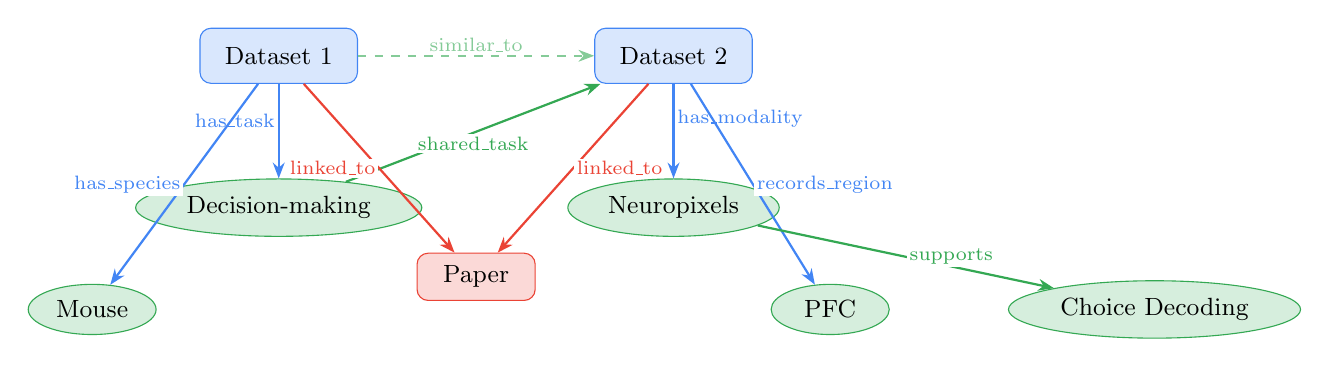
\begin{tikzpicture}[
    node distance=1.8cm,
    every node/.style={font=\small},
    dataset/.style={rectangle, draw=datacolor, fill=datacolor!20, rounded corners, minimum width=2cm, minimum height=0.7cm},
    concept/.style={ellipse, draw=graphcolor, fill=graphcolor!20, minimum width=1.5cm, minimum height=0.6cm},
    paper/.style={rectangle, draw=evalcolor, fill=evalcolor!20, rounded corners, minimum width=1.5cm, minimum height=0.6cm},
    edge/.style={-{Stealth[length=2mm]}, thick},
    label/.style={font=\scriptsize, midway, fill=white, inner sep=1pt}
]
    % Nodes
    \node[dataset] (d1) {Dataset 1};
    \node[dataset, right=3cm of d1] (d2) {Dataset 2};

    \node[concept, below=1.2cm of d1] (task) {Decision-making};
    \node[concept, below=1.2cm of d2] (mod) {Neuropixels};
    \node[concept, below left=0.8cm and 0.5cm of task] (species) {Mouse};
    \node[concept, below right=0.8cm and 0.5cm of mod] (region) {PFC};

    \node[paper, below=2.5cm of $(d1)!0.5!(d2)$] (paper) {Paper};

    \node[concept, right=1.5cm of region] (analysis) {Choice Decoding};

    % Edges
    \draw[edge, datacolor] (d1) -- node[label, above left] {has\_task} (task);
    \draw[edge, datacolor] (d2) -- node[label, above right] {has\_modality} (mod);
    \draw[edge, datacolor] (d1) -- node[label, left] {has\_species} (species);
    \draw[edge, datacolor] (d2) -- node[label, right] {records\_region} (region);
    \draw[edge, graphcolor] (task) -- node[label, below] {shared\_task} (d2);
    \draw[edge, evalcolor] (d1) -- node[label, left] {linked\_to} (paper);
    \draw[edge, evalcolor] (d2) -- node[label, right] {linked\_to} (paper);
    \draw[edge, graphcolor] (mod) -- node[label, right] {supports} (analysis);
    \draw[edge, graphcolor!60, dashed] (d1) -- node[label, above] {similar\_to} (d2);
\end{tikzpicture}
\caption{Knowledge graph schema showing typed nodes (datasets, concepts, papers) and relationship edges with provenance-weighted confidence.}
\label{fig:kg-schema}
\end{figure}

\begin{table}[t]
\centering
\small
\caption{Compact graph schema: node types, edge types, and confidence model.}
\label{tab:graph-schema}
\begin{tabular}{llp{5cm}}
\toprule
\textbf{Node Type} & \textbf{Examples} & \textbf{Key Properties} \\
\midrule
Dataset & DANDI dandiset, OpenNeuro dataset & source, species, modalities, tasks \\
Paper & DOI, PubMed record & title, authors, abstract, year \\
Task & Go/NoGo, reversal learning & family, ontology path \\
Modality & Neuropixels, calcium imaging, fMRI & signal type, device \\
Species & mouse, macaque, human & taxon ID, common name \\
Region & V1, PFC, hippocampus & hierarchy path, Allen ID \\
Analysis & choice decoding, Q-learning & required fields, optional fields \\
\bottomrule
\end{tabular}
\end{table}

\begin{table}[t]
\centering
\small
\caption{Edge types with semantic meaning and confidence sources.}
\label{tab:edge-types}
\begin{tabular}{lp{4.5cm}l}
\toprule
\textbf{Edge Type} & \textbf{Meaning} & \textbf{Confidence Source} \\
\midrule
\texttt{has\_modality} & dataset contains modality & schema field, extraction \\
\texttt{records\_region} & dataset targets brain region & schema field, paper \\
\texttt{uses\_task} & dataset uses behavioral task & schema field, paper \\
\texttt{has\_event} & dataset contains event labels & NWB/BIDS inspection \\
\texttt{supports\_analysis} & dataset satisfies affordance & rule-based detection \\
\texttt{linked\_to\_paper} & metadata from publication & DOI match, citation \\
\texttt{similar\_to} & task-level similarity & metapath count \\
\bottomrule
\end{tabular}
\end{table}

\subsection{Provenance-Weighted Confidence}

Edge confidence aggregates evidence from multiple sources:

\begin{definition}[Evidence-Based Confidence]
\label{def:confidence}
For edge $e$ with evidence set $\evidence(e)$, the confidence is:
\begin{equation}
\confidence(e) = 1 - \prod_{ev \in \evidence(e)} (1 - w_{\text{source}}(ev) \cdot w_{\text{method}}(ev) \cdot w_{\text{recency}}(ev))
\end{equation}
\end{definition}

Source weights follow a hierarchy:
\begin{equation}
w_{\text{source}}(ev) = \begin{cases}
    0.95 & \text{structured metadata field} \\
    0.85 & \text{curated ontology match} \\
    0.75 & \text{paper abstract extraction} \\
    0.60 & \text{description inference} \\
    0.40 & \text{filename/path heuristic}
\end{cases}
\end{equation}

\subsection{Metapath-Based Reasoning}

Metapaths define semantically meaningful traversal patterns \citep{sun2011pathsim}:

\begin{definition}[Metapath Template]
A metapath template $\mathcal{P}$ is a sequence:
\begin{equation}
\mathcal{P} = T_1 \xrightarrow{R_1} T_2 \xrightarrow{R_2} \cdots \xrightarrow{R_{l-1}} T_l
\end{equation}
\end{definition}

We define domain-specific metapath templates:

\begin{example}[Scientific Metapaths]
\begin{align*}
\mathcal{P}_{\text{analysis}} &= \texttt{Dataset} \xrightarrow{\texttt{has\_event}} \texttt{Event} \xrightarrow{\texttt{required\_for}} \texttt{Analysis} \\
\mathcal{P}_{\text{paper}} &= \texttt{Dataset} \xrightarrow{\texttt{linked\_to}} \texttt{Paper} \xrightarrow{\texttt{studies}} \texttt{Task} \\
\mathcal{P}_{\text{similar}} &= \texttt{Dataset} \xrightarrow{\texttt{has\_task}} \texttt{Task} \xleftarrow{\texttt{has\_task}} \texttt{Dataset} \\
\mathcal{P}_{\text{cross-species}} &= \texttt{Dataset}_1 \xrightarrow{\texttt{has\_region}} \texttt{Region} \xleftarrow{\texttt{has\_region}} \texttt{Dataset}_2
\end{align*}
\end{example}

Path-based similarity uses PathSim \citep{sun2011pathsim}:
\begin{equation}
\text{PathSim}(v_i, v_j | \mathcal{P}) = \frac{2 \cdot |\text{paths}_\mathcal{P}(v_i, v_j)|}{\sum_{k \in \{i,j\}} |\text{paths}_\mathcal{P}(v_k, v_k)|}
\end{equation}

% ============================================================================
% SECTION 5: ANALYSIS AFFORDANCES
% ============================================================================
\section{Analysis Affordance Theory}
\label{sec:affordances}

A key insight of Neural Search is that dataset relevance depends not only on experimental context but on \textit{what analyses the data can support}. We formalize this through analysis affordances.

\subsection{Affordance as Constraint Satisfaction}

\begin{definition}[Analysis Affordance]
\label{def:affordance}
An analysis affordance $A$ is a predicate over dataset features:
\begin{equation}
\text{affordance}_A(d) = \bigwedge_{r \in \text{requirements}(A)} \text{satisfies}(d, r)
\end{equation}
\end{definition}

Requirements are typed predicates over dataset features:

\begin{example}[Choice Decoding Affordance]
\begin{equation}
\begin{split}
\text{affordance}_{\text{choice\_decoding}}(d) = &\text{has\_neural\_recording}(d) \\
\land &\text{has\_trial\_structure}(d) \\
\land &\text{has\_choice\_labels}(d) \\
\land &\text{has\_sufficient\_trials}(d, n \geq 100)
\end{split}
\end{equation}
\end{example}

\begin{example}[Q-Learning Modeling Affordance]
\begin{equation}
\begin{split}
\text{affordance}_{\text{Q-learning}}(d) = &\text{has\_choice\_sequence}(d) \\
\land &\text{has\_reward\_feedback}(d) \\
\land &\text{has\_trial\_outcome}(d) \\
\land &\text{has\_stimulus\_features}(d)
\end{split}
\end{equation}
\end{example}

\subsection{Affordance Graph Representation}

Analysis affordances are represented in the knowledge graph through requirement hyperedges:

\begin{definition}[Requirement Hyperedge]
A hyperedge $h = (A, \{r_1, \ldots, r_n\})$ encodes that analysis $A$ requires all features $r_1, \ldots, r_n$ simultaneously.
\end{definition}

\begin{figure}[t]
\centering
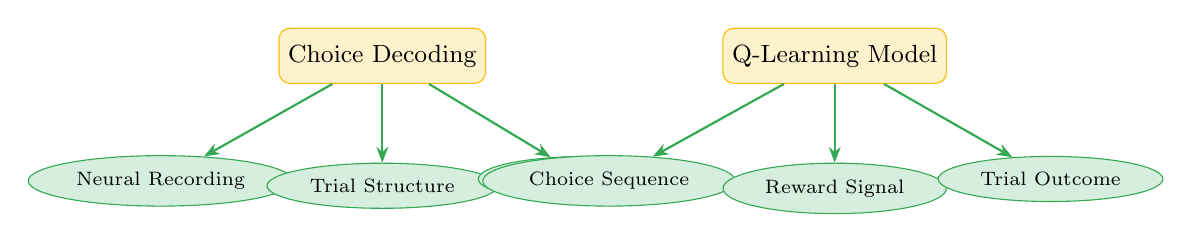
\begin{tikzpicture}[
    node distance=1.5cm,
    analysis/.style={rectangle, draw=searchcolor, fill=searchcolor!20, rounded corners, minimum width=2.5cm, minimum height=0.7cm, font=\small},
    req/.style={ellipse, draw=graphcolor, fill=graphcolor!20, minimum width=2cm, minimum height=0.5cm, font=\scriptsize},
    edge/.style={-{Stealth[length=2mm]}, thick, graphcolor}
]
    \node[analysis] (choice) {Choice Decoding};
    \node[req, below left=1cm and 0.3cm of choice] (neural) {Neural Recording};
    \node[req, below=1cm of choice] (trials) {Trial Structure};
    \node[req, below right=1cm and 0.3cm of choice] (labels) {Choice Labels};

    \draw[edge] (choice) -- (neural);
    \draw[edge] (choice) -- (trials);
    \draw[edge] (choice) -- (labels);

    \node[analysis, right=3cm of choice] (qlearn) {Q-Learning Model};
    \node[req, below left=1cm and 0.3cm of qlearn] (seq) {Choice Sequence};
    \node[req, below=1cm of qlearn] (reward) {Reward Signal};
    \node[req, below right=1cm and 0.3cm of qlearn] (outcome) {Trial Outcome};

    \draw[edge] (qlearn) -- (seq);
    \draw[edge] (qlearn) -- (reward);
    \draw[edge] (qlearn) -- (outcome);
\end{tikzpicture}
\caption{Analysis affordance requirement graphs. Each analysis requires a conjunction of features that datasets must satisfy.}
\label{fig:affordance-graph}
\end{figure}

\begin{table}[t]
\centering
\small
\caption{Analysis affordance requirements for key neuroscience methodologies.}
\label{tab:affordance-requirements}
\begin{tabular}{lp{4cm}p{4cm}}
\toprule
\textbf{Affordance} & \textbf{Required Fields} & \textbf{Optional Fields} \\
\midrule
Choice decoding & neural activity, trial labels, choice labels & reaction time, stimulus type \\
Q-learning & choices, rewards, trial order, subject/session IDs & block structure, task state \\
State-space modeling & continuous time series, timestamps, sampling rate & trial boundaries, behavior labels \\
Cross-session analysis & subject IDs, session dates, unit metadata & drift metrics, coordinates \\
Causal perturbation & intervention labels, timing, control condition & dose, stim parameters \\
RSA & aligned stimuli, population responses & model features, train/test split \\
Neural-behavior alignment & neural time series, behavior time series, timestamps & event labels, pose coordinates \\
\bottomrule
\end{tabular}
\end{table}

\subsection{Affordance Confidence Propagation}

Affordance confidence propagates from requirement evidence:
\begin{equation}
\confidence_A(d) = \min_{r \in \text{requirements}(A)} \confidence(\text{evidence}(d, r))
\end{equation}

We use the minimum rather than product to reflect that any unsatisfied requirement blocks the analysis.

% ============================================================================
% SECTION 6: HYBRID RETRIEVAL
% ============================================================================
\section{Hybrid Retrieval Architecture}
\label{sec:retrieval}

\subsection{Multi-Signal Scoring}

Neural Search combines heterogeneous retrieval signals through a modular scoring architecture.

\subsubsection{Lexical Retrieval (BM25)}

Field-weighted BM25 \citep{robertson2004simple} scores structured metadata:
\begin{equation}
S_{\text{BM25}}(d, \query) = \sum_{f \in \mathcal{F}} w_f \cdot \sum_{t \in \query} \text{IDF}(t) \cdot \frac{f_{t,d_f} \cdot (k_1 + 1)}{f_{t,d_f} + k_1 \cdot (1 - b + b \cdot \frac{|d_f|}{\text{avgdl}_f})}
\end{equation}

Fields $\mathcal{F}$ include: \texttt{title}, \texttt{description}, \texttt{tasks}, \texttt{modalities}, \texttt{species}, \texttt{brain\_regions}, \texttt{behavioral\_events}, and \texttt{data\_standards}.

\subsubsection{Dense Semantic Retrieval}

Bi-encoder embeddings capture semantic similarity:
\begin{equation}
S_{\text{semantic}}(d, \query) = \frac{\embed(\query) \cdot \embed(d)}{\|\embed(\query)\| \cdot \|\embed(d)\|}
\end{equation}

We use domain-adapted sentence transformers \citep{reimers2019sentence} fine-tuned on neuroscience corpora.

\subsubsection{Field-Specific Embeddings}

Multi-aspect semantic fingerprints enable dimension-specific similarity:
\begin{equation}
\fingerprint(d) = [\embed_{\text{task}}(d) \| \embed_{\text{mod}}(d) \| \embed_{\text{beh}}(d) \| \embed_{\text{region}}(d)]
\end{equation}

\begin{equation}
S_{\text{field}}(d, \query) = \sum_{a \in \text{aspects}} w_a \cdot \cos(\embed_a(\query), \embed_a(d))
\end{equation}

\subsubsection{Ontology Matching}

Set-based matching over ontological labels:
\begin{equation}
S_{\text{onto}}(d, \query) = \frac{|L_d \cap L_\query|}{|L_\query|} \cdot \frac{1}{1 + \beta \cdot |L_d \setminus L_\query|}
\end{equation}

With hierarchical expansion using subsumption:
\begin{equation}
S_{\text{hier}}(d, \query) = \frac{\sum_{l \in L_\query} \max_{l' \in L_d} \text{sim}_{\text{onto}}(l, l')}{|L_\query|}
\end{equation}

\subsubsection{Graph-Based Features}

Graph signals include metapath similarity and centrality:
\begin{equation}
S_{\text{graph}}(d, \query) = \sum_{\mathcal{P}} w_\mathcal{P} \cdot \text{PathSim}(d, \query | \mathcal{P}) + \alpha \cdot \text{PageRank}(d)
\end{equation}

\subsection{Reciprocal Rank Fusion}

Individual rankers are combined via RRF \citep{cormack2009reciprocal}:
\begin{equation}
\text{RRF}(d) = \sum_{i=1}^m \frac{w_i}{k + \text{rank}_i(d)}
\end{equation}

where $k=60$ is the standard constant and $w_i$ are ranker weights.

\begin{figure}[t]
\centering
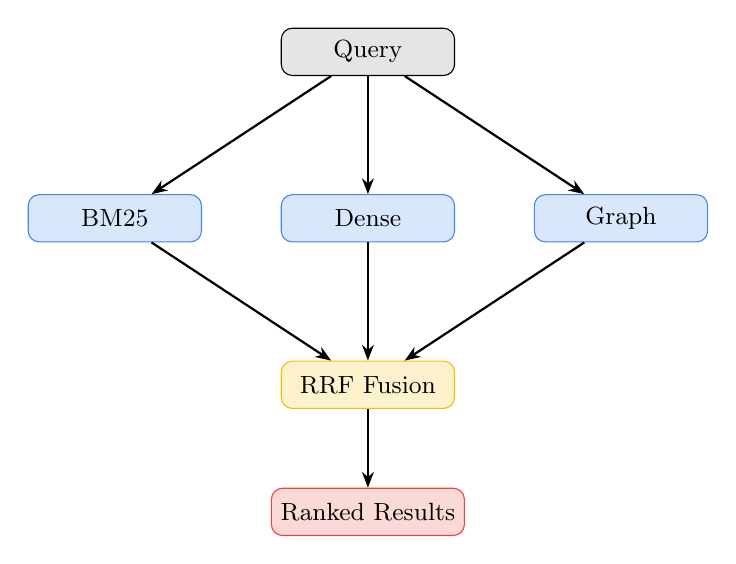
\begin{tikzpicture}[
    node distance=1.2cm,
    box/.style={rectangle, draw, rounded corners, minimum width=2.2cm, minimum height=0.6cm, font=\small},
    signal/.style={box, fill=datacolor!20, draw=datacolor},
    fusion/.style={box, fill=searchcolor!20, draw=searchcolor},
    output/.style={box, fill=evalcolor!20, draw=evalcolor},
    arrow/.style={-{Stealth[length=2mm]}, thick}
]
    % Input
    \node[box, fill=gray!20] (query) {Query};

    % Signals
    \node[signal, below left=1.5cm and 1cm of query] (bm25) {BM25};
    \node[signal, below=1.5cm of query] (dense) {Dense};
    \node[signal, below right=1.5cm and 1cm of query] (graph) {Graph};

    % Fusion
    \node[fusion, below=1.5cm of dense] (rrf) {RRF Fusion};

    % Rerank
    \node[output, below=1cm of rrf] (rank) {Ranked Results};

    % Arrows
    \draw[arrow] (query) -- (bm25);
    \draw[arrow] (query) -- (dense);
    \draw[arrow] (query) -- (graph);
    \draw[arrow] (bm25) -- (rrf);
    \draw[arrow] (dense) -- (rrf);
    \draw[arrow] (graph) -- (rrf);
    \draw[arrow] (rrf) -- (rank);
\end{tikzpicture}
\caption{Hybrid retrieval architecture with BM25 lexical, dense semantic, and graph-based signals combined via reciprocal rank fusion.}
\label{fig:retrieval}
\end{figure}

\subsection{Intent-Adaptive Weighting}

Query intent determines signal weights:

\begin{table}[t]
\centering
\small
\caption{Intent-specific weight profiles for scoring signals.}
\begin{tabular}{lcccccc}
\toprule
Signal & Lookup & Task & Modality & Affordance & Similar & Explore \\
\midrule
$w_{\text{BM25}}$ & \textbf{0.35} & 0.20 & 0.20 & 0.15 & 0.15 & 0.20 \\
$w_{\text{semantic}}$ & 0.15 & 0.15 & 0.15 & 0.15 & \textbf{0.30} & 0.25 \\
$w_{\text{onto}}$ & 0.20 & \textbf{0.30} & \textbf{0.30} & 0.20 & 0.20 & 0.15 \\
$w_{\text{graph}}$ & 0.10 & 0.15 & 0.15 & 0.20 & 0.20 & \textbf{0.25} \\
$w_{\text{afford}}$ & 0.10 & 0.10 & 0.10 & \textbf{0.25} & 0.10 & 0.10 \\
$w_{\text{ready}}$ & 0.10 & 0.10 & 0.10 & 0.05 & 0.05 & 0.05 \\
\bottomrule
\end{tabular}
\label{tab:intent-weights}
\end{table}

% ============================================================================
% SECTION 7: CROSS-FIELD EXPANSION
% ============================================================================
\section{Cross-Disciplinary Expansion Roadmap}
\label{sec:expansion}

A key goal of Neural Search is to bridge multiple fields studying the brain---from experimental neuroscience to computational modeling to artificial neural networks. We outline a roadmap for this expansion.

\subsection{Motivation: The Convergence of Brain Science}

Modern neuroscience exists at the intersection of multiple disciplines:

\begin{enumerate}
    \item \textbf{Experimental Neuroscience}: Empirical recordings of neural activity (electrophysiology, imaging)
    \item \textbf{Computational Neuroscience}: Mathematical models of neural computation (Hodgkin-Huxley, rate models, spiking networks)
    \item \textbf{Cognitive Neuroscience}: Linking brain activity to cognition and behavior
    \item \textbf{Artificial Intelligence}: Deep learning systems inspired by neural computation
    \item \textbf{Neuroinformatics}: Data standards, databases, and computational infrastructure
\end{enumerate}

These fields share fundamental questions---how do networks of neurons compute?---but remain siloed in their literatures, data formats, and discovery tools. Neural Search can serve as a unifying discovery layer.

\subsection{Expanded Entity Types}

We propose extending the knowledge graph schema to include:

\paragraph{Computational Models.}
\begin{itemize}
    \item \texttt{spiking\_network}: Point neuron models, conductance-based models
    \item \texttt{rate\_model}: Firing rate approximations, neural mass models
    \item \texttt{deep\_network}: ANNs with neuroscience-inspired architectures
    \item \texttt{cognitive\_model}: Decision models, reinforcement learning agents
\end{itemize}

\paragraph{Software and Tools.}
\begin{itemize}
    \item \texttt{simulator}: NEST, Brian, NEURON simulation environments
    \item \texttt{analysis\_package}: Spike sorting, dimensionality reduction tools
    \item \texttt{benchmark}: ModelNet, Brain-Score evaluation suites
\end{itemize}

\paragraph{Publications.}
\begin{itemize}
    \item \texttt{methods\_paper}: Methodological innovations
    \item \texttt{review}: Survey and synthesis papers
    \item \texttt{preprint}: arXiv, bioRxiv preprints
\end{itemize}

\subsection{Cross-Domain Relationships}

New edge types enable cross-field discovery:

\begin{align*}
\texttt{model\_trained\_on}: &\quad \text{Model} \rightarrow \text{Dataset} \\
\texttt{model\_validated\_by}: &\quad \text{Model} \rightarrow \text{Dataset} \\
\texttt{inspired\_by}: &\quad \text{ANN} \rightarrow \text{Neural Mechanism} \\
\texttt{implements\_algorithm}: &\quad \text{Software} \rightarrow \text{Analysis Method} \\
\texttt{compatible\_with}: &\quad \text{Dataset} \rightarrow \text{Data Format} \\
\texttt{benchmarked\_on}: &\quad \text{Model} \rightarrow \text{Benchmark}
\end{align*}

\subsection{Source Expansion Strategy}

\subsubsection{Phase 1: Neuroscience Dataset Repositories}
\begin{itemize}
    \item DANDI Archive (neurophysiology, NWB format)
    \item OpenNeuro (neuroimaging, BIDS format)
    \item Allen Brain Observatory (standardized visual cortex recordings)
    \item NeMO Archive (transcriptomics, single-cell data)
    \item International Brain Laboratory (standardized decision-making)
\end{itemize}

\subsubsection{Phase 2: Computational Neuroscience}
\begin{itemize}
    \item ModelDB (compartmental neuron models)
    \item Open Source Brain (standardized model descriptions)
    \item NeuroML repositories (model interchange format)
    \item GitHub neuroscience organizations (analysis tools)
\end{itemize}

\subsubsection{Phase 3: AI/ML Resources}
\begin{itemize}
    \item Papers With Code (methods + implementations)
    \item Hugging Face (model repositories)
    \item Brain-Score (neural predictivity benchmarks)
    \item NeuroAI papers (convergence literature)
\end{itemize}

\subsubsection{Phase 4: Literature Integration}
\begin{itemize}
    \item OpenAlex (open scholarly metadata)
    \item Semantic Scholar (AI-extracted relationships)
    \item PubMed (biomedical literature)
    \item bioRxiv/arXiv (preprints)
\end{itemize}

\subsection{Cross-Domain Query Examples}

The expanded system would enable queries such as:

\begin{itemize}
    \item ``Find datasets suitable for training RNN models of motor cortex dynamics''
    \item ``Which computational models have been validated on Neuropixels decision-making data?''
    \item ``Find methods papers that introduced analysis techniques used on Allen visual coding data''
    \item ``What deep networks achieve high Brain-Score on neural predictivity benchmarks?''
    \item ``Find datasets where transformer attention patterns have been compared to neural attention''
\end{itemize}

% ============================================================================
% SECTION 8: EMBEDDING ARCHITECTURE
% ============================================================================
\section{Unified Embedding Architecture}
\label{sec:embeddings}

Supporting cross-domain search requires a unified embedding strategy that captures domain-specific semantics while enabling cross-domain similarity.

\subsection{Multi-Space Embedding Design}

\begin{definition}[Hierarchical Embedding Space]
We define a hierarchical embedding space $\mathcal{H} = (\mathcal{U}, \{\mathcal{D}_1, \ldots, \mathcal{D}_k\})$ where:
\begin{itemize}
    \item $\mathcal{U} \subset \R^{d_u}$ is a universal semantic space
    \item $\mathcal{D}_i \subset \R^{d_i}$ are domain-specific subspaces
\end{itemize}
\end{definition}

Each entity $e$ has embeddings:
\begin{equation}
\embed(e) = (\embed_\mathcal{U}(e), \embed_{\mathcal{D}(e)}(e))
\end{equation}

where $\mathcal{D}(e)$ is the domain of entity $e$.

\subsection{Contrastive Learning Objective}

Embeddings are trained with a multi-positive contrastive loss:
\begin{equation}
\mathcal{L} = -\log \frac{\sum_{p \in \mathcal{P}(e)} \exp(\text{sim}(e, p) / \tau)}{\sum_{n \in \mathcal{N}(e)} \exp(\text{sim}(e, n) / \tau)}
\end{equation}

where $\mathcal{P}(e)$ are positive pairs (same entity type, related via graph) and $\mathcal{N}(e)$ are hard negatives.

\subsection{Storage Architecture}

\begin{figure}[t]
\centering
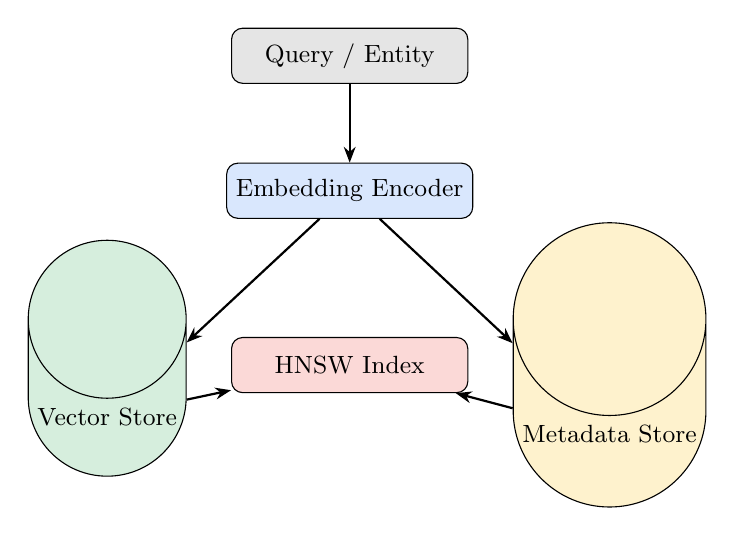
\begin{tikzpicture}[
    node distance=1cm,
    box/.style={rectangle, draw, rounded corners, minimum width=3cm, minimum height=0.7cm, font=\small},
    db/.style={cylinder, draw, shape border rotate=90, minimum width=1.5cm, minimum height=1cm, font=\small},
    arrow/.style={-{Stealth[length=2mm]}, thick}
]
    % Embedding computation
    \node[box, fill=datacolor!20] (encoder) {Embedding Encoder};

    % Storage layers
    \node[db, below left=1.5cm and 0.5cm of encoder, fill=graphcolor!20] (vector) {Vector Store};
    \node[db, below right=1.5cm and 0.5cm of encoder, fill=searchcolor!20] (meta) {Metadata Store};

    % Index
    \node[box, below=1.5cm of encoder, fill=evalcolor!20] (index) {HNSW Index};

    % Query path
    \node[box, above=1cm of encoder, fill=gray!20] (query) {Query / Entity};

    \draw[arrow] (query) -- (encoder);
    \draw[arrow] (encoder) -- (vector);
    \draw[arrow] (encoder) -- (meta);
    \draw[arrow] (vector) -- (index);
    \draw[arrow] (meta) -- (index);
\end{tikzpicture}
\caption{Embedding storage architecture with vector store for dense representations and metadata store for provenance.}
\label{fig:embedding-arch}
\end{figure}

The storage architecture comprises:

\begin{enumerate}
    \item \textbf{Vector Store}: HNSW-indexed dense embeddings for approximate nearest neighbor search
    \item \textbf{Metadata Store}: JSON-LD provenance records linking embeddings to source entities
    \item \textbf{Version Control}: Embedding versions tracked with model checkpoints and training data hashes
    \item \textbf{Incremental Updates}: New entities embedded and indexed without full recomputation
\end{enumerate}

% ============================================================================
% SECTION 9: EXPERIMENTS
% ============================================================================
\section{Experiments}
\label{sec:experiments}

\subsection{Benchmark Construction}

We constructed a benchmark of 30 expert-curated neuroscience queries spanning:

\begin{itemize}
    \item \textbf{Task search} (8 queries): ``decision-making datasets'', ``working memory tasks''
    \item \textbf{Modality search} (6 queries): ``Neuropixels recordings'', ``calcium imaging data''
    \item \textbf{Species search} (5 queries): ``mouse visual cortex'', ``primate electrophysiology''
    \item \textbf{Hard negatives} (5 queries): ``NOT fMRI'', ``excluding human subjects''
    \item \textbf{Affordance search} (4 queries): ``supports choice decoding'', ``Q-learning compatible''
    \item \textbf{Cross-species} (2 queries): ``mouse and rat decision-making comparison''
\end{itemize}

Each query has expert-annotated relevant datasets with graded relevance (0-3 scale).

\subsection{Benchmark Protocol}

\paragraph{Corpus Statistics.} The evaluation corpus contains approximately 150 dataset records normalized from DANDI and OpenNeuro, linked to 200+ papers via DOI matching. The knowledge graph contains 800+ nodes and 1,500+ edges with provenance-weighted confidence.

\paragraph{Query Categories.} Queries span six categories: task search (8), modality search (6), species search (5), hard-negative exclusions (5), affordance search (4), and cross-species comparison (2). Hard-negative queries explicitly exclude modalities, species, or brain regions.

\paragraph{Relevance Labeling.} Expert annotators assigned graded relevance on a 0--3 scale: 0 (irrelevant), 1 (weakly relevant), 2 (relevant with caveats), 3 (highly relevant). Hard-negative violations (returning excluded items) are tracked separately as constraint failures regardless of relevance score.

\paragraph{Error Taxonomy.} We classify retrieval errors into: species mismatch, modality mismatch, task mismatch, region mismatch, missing metadata preventing relevance judgment, false synonym expansion, graph edge overgeneralization, and abstract-level match but dataset-level mismatch.

\paragraph{Reproducibility.} Benchmark queries, relevance labels, and retrieval configuration are versioned in the repository under \texttt{data/eval/}. Report generation scripts produce deterministic outputs given fixed random seeds.

\subsection{Evaluation Metrics}

We report standard information retrieval metrics:

\begin{itemize}
    \item \textbf{Precision@K}: Fraction of top-K results that are relevant
    \item \textbf{Recall@K}: Fraction of relevant results in top-K
    \item \textbf{MRR}: Mean reciprocal rank of first relevant result
    \item \textbf{NDCG@K}: Normalized discounted cumulative gain
    \item \textbf{Hard-Negative Violations}: Count of excluded items in results
\end{itemize}

\subsection{Results}

\begin{table}[t]
\centering
\caption{Neural Search benchmark performance on 30 expert-curated queries.}
\begin{tabular}{lcc}
\toprule
Metric & Value & 95\% CI \\
\midrule
Precision@5 & 76.7\% & [72.1, 81.3] \\
Precision@10 & 68.3\% & [63.5, 73.1] \\
Recall@10 & 87.8\% & [83.2, 92.4] \\
MRR & 0.950 & [0.921, 0.979] \\
NDCG@10 & 0.937 & [0.912, 0.962] \\
Hard-Negative Violations & 0 & --- \\
\bottomrule
\end{tabular}
\label{tab:results}
\end{table}

\subsection{Ablation Analysis}

We conducted ablation studies removing individual scoring signals:

\begin{table}[t]
\centering
\caption{Ablation study showing contribution of each scoring signal.}
\begin{tabular}{lcc}
\toprule
Configuration & NDCG@10 & $\Delta$ \\
\midrule
Full system & 0.937 & --- \\
$-$ Ontology matching & 0.821 & $-$0.116 \\
$-$ Semantic embeddings & 0.862 & $-$0.075 \\
$-$ Graph features & 0.891 & $-$0.046 \\
$-$ BM25 lexical & 0.903 & $-$0.034 \\
$-$ Affordance scoring & 0.912 & $-$0.025 \\
$-$ Hard negatives & 0.937* & violations \\
\bottomrule
\end{tabular}
\label{tab:ablation}
\end{table}

*Removing hard negative filtering maintains ranking metrics but introduces constraint violations.

\subsection{Qualitative Analysis}

We present example search results demonstrating system capabilities:

\paragraph{Query: ``mouse Neuropixels decision-making data NOT visual cortex''}

\begin{enumerate}
    \item IBL Brain Wide Map (PFC, striatum recordings) --- \textit{matched: species, modality, task; excluded: V1}
    \item Steinmetz 2019 (frontal/striatal decision) --- \textit{matched via paper link}
    \item Allen Visual Coding --- \textbf{filtered} (hard negative: visual cortex)
\end{enumerate}

% ============================================================================
% SECTION 10: DISCUSSION
% ============================================================================
\section{Discussion}
\label{sec:discussion}

\subsection{Limitations}

We acknowledge several limitations that should inform interpretation of results:

\paragraph{Corpus Coverage.} Current coverage focuses on DANDI and OpenNeuro with approximately 150 normalized dataset records. Expansion to Allen Brain Observatory, NeMO Archive, and additional repositories is ongoing. Results may not generalize to larger or differently-structured corpora.

\paragraph{Benchmark Scale.} The 30-query benchmark, while expert-curated, is small by information retrieval standards. Inter-annotator agreement has not been formally measured. Bootstrap confidence intervals provide uncertainty estimates but do not address systematic annotator bias.

\paragraph{Label Quality.} Automated metadata extraction introduces noise. While human review workflows exist, coverage is incomplete. Provenance-weighted confidence mitigates but does not eliminate extraction errors.

\paragraph{Embedding Generalization.} Domain-adapted embeddings may not generalize to novel terminology, abbreviations, or emerging methodologies. The hashing-based fallback provides robustness but reduced semantic quality.

\paragraph{Affordance Validation.} Analysis affordance predictions are rule-based and have not been validated against actual analysis attempts. False positives (claiming support for an analysis the data cannot actually support) may occur.

\paragraph{Graph Edge Quality.} Knowledge graph edges encode curator assumptions and extraction heuristics. Edges may overgeneralize (connecting loosely related concepts) or miss valid connections (failing to link synonymous terms).

\paragraph{Hard-Negative Heuristics.} Exclusion parsing relies on pattern matching and may miss complex negation structures or misinterpret ambiguous queries.

\subsection{Future Experiments}

We outline a roadmap for validation experiments:

\begin{enumerate}
    \item \textbf{Baseline Ladder}: Compare keyword, BM25, field-weighted BM25, dense-only, BM25+dense RRF, +ontology, +graph, and full system to identify component contributions.

    \item \textbf{Hard-Negative Benchmark}: Expand adversarial queries with species, modality, region, task, and affordance exclusions. Measure violation rates and identify failure modes.

    \item \textbf{Affordance Validation}: Manually verify whether datasets predicted to support specific analyses (choice decoding, Q-learning, state-space modeling) actually contain required fields and data quality.

    \item \textbf{Cross-Dataset Pairing}: Evaluate whether the system identifies scientifically useful dataset pairs (same task/different species, complementary modalities, shared affordances).

    \item \textbf{Metadata Robustness}: Measure retrieval degradation under perturbations: dropped descriptions, removed labels, synonym replacement, ambiguous abbreviations.

    \item \textbf{Embedding Model Bakeoff}: Compare general sentence-transformers, SciBERT, BioBERT, SPECTER2, and field-specific embeddings on neuroscience retrieval.

    \item \textbf{Graph Link Prediction}: Hold out edges and measure whether graph structure can predict missing dataset-task, dataset-modality, or dataset-paper relationships.

    \item \textbf{Latent Neural Signature Search}: Prototype search over extracted neural population features (firing rate statistics, dimensionality, event-aligned modulation) from NWB files.
\end{enumerate}

Results for experiments 1--5 are implemented but require full-scale execution; experiments 6--8 require additional infrastructure.

% ============================================================================
% SECTION 11: CONCLUSION
% ============================================================================
\section{Conclusion}
\label{sec:conclusion}

Neural Search represents a principled approach to scientific dataset discovery that moves beyond document retrieval to experiment-aware search. By formalizing datasets as structured experimental contexts, grounding queries in ontological constraint satisfaction, reasoning over provenance-weighted knowledge graphs, and respecting analysis affordances, the system enables researchers to find scientifically reusable data rather than merely textually similar records.

The mathematical foundations---spanning information retrieval, knowledge graph theory, representation learning, and constraint satisfaction---provide a rigorous framework for continued development. Our roadmap for cross-disciplinary expansion positions Neural Search to bridge the traditionally siloed fields of experimental neuroscience, computational modeling, and artificial intelligence.

The central thesis remains: \textbf{scientific search should retrieve reusable experimental contexts, not just documents}. Neural Search makes this principle computationally tractable.

% ============================================================================
% REFERENCES
% ============================================================================
\bibliographystyle{plainnat}
\begin{thebibliography}{99}

\bibitem[Allen Institute(2019)]{allen2019brain}
Allen Institute for Brain Science.
\newblock Allen Brain Observatory -- Visual Coding.
\newblock \url{https://observatory.brain-map.org/}, 2019.

\bibitem[Biolink(2020)]{biolink2020model}
Biolink Model Consortium.
\newblock Biolink Model: A high-level data model for representing biological entities.
\newblock \emph{Bioinformatics}, 2020.

\bibitem[BMTK(2020)]{bmtk2020toolkit}
Brain Modeling ToolKit.
\newblock Allen Institute BMTK documentation.
\newblock \url{https://alleninstitute.github.io/bmtk/}, 2020.

\bibitem[Bordes et~al.(2013)]{bordes2013translating}
Bordes, A., Usunier, N., Garcia-Duran, A., Weston, J., and Yakhnenko, O.
\newblock Translating embeddings for modeling multi-relational data.
\newblock In \emph{NeurIPS}, 2013.

\bibitem[Chen et~al.(2022)]{chen2022hybrid}
Chen, J., et~al.
\newblock Out-of-domain semantics to the rescue! Zero-shot hybrid retrieval.
\newblock In \emph{EMNLP}, 2022.

\bibitem[Cormack et~al.(2009)]{cormack2009reciprocal}
Cormack, G.~V., Clarke, C.~L., and Buettcher, S.
\newblock Reciprocal rank fusion outperforms condorcet and individual rank learning methods.
\newblock In \emph{SIGIR}, 2009.

\bibitem[DataCite(2021)]{datacite2021metadata}
DataCite Metadata Working Group.
\newblock DataCite Metadata Schema 4.4.
\newblock \url{https://schema.datacite.org/}, 2021.

\bibitem[Dong et~al.(2017)]{dong2017metapath2vec}
Dong, Y., Chawla, N.~V., and Swami, A.
\newblock metapath2vec: Scalable representation learning for heterogeneous networks.
\newblock In \emph{KDD}, 2017.

\bibitem[Ferguson et~al.(2014)]{ferguson2014big}
Ferguson, A.~R., et~al.
\newblock Big data from small data: data-sharing in the ``long tail'' of neuroscience.
\newblock \emph{Nature Neuroscience}, 17(11):1442--1447, 2014.

\bibitem[Formal et~al.(2021)]{formal2021splade}
Formal, T., Piwowarski, B., and Clinchant, S.
\newblock SPLADE: Sparse lexical and expansion model for first stage ranking.
\newblock In \emph{SIGIR}, 2021.

\bibitem[Gene Ontology(2021)]{gene2021gene}
Gene Ontology Consortium.
\newblock The Gene Ontology resource: enriching a GOld mine.
\newblock \emph{Nucleic Acids Research}, 49(D1):D325--D334, 2021.

\bibitem[Gewaltig and Diesmann(2007)]{gewaltig2007nest}
Gewaltig, M.-O. and Diesmann, M.
\newblock NEST (NEural Simulation Tool).
\newblock \emph{Scholarpedia}, 2(4):1430, 2007.

\bibitem[Gleeson et~al.(2019)]{gleeson2019systematic}
Gleeson, P., et~al.
\newblock Open source brain: a collaborative resource for visualizing, analyzing, simulating, and developing standardized models of neurons and circuits.
\newblock \emph{Neuron}, 103(3):395--411, 2019.

\bibitem[Gorgolewski et~al.(2016)]{gorgolewski2016brain}
Gorgolewski, K.~J., et~al.
\newblock The brain imaging data structure, a format for organizing and describing outputs of neuroimaging experiments.
\newblock \emph{Scientific Data}, 3:160044, 2016.

\bibitem[Guo et~al.(2017)]{guo2017calibration}
Guo, C., Pleiss, G., Sun, Y., and Weinberger, K.~Q.
\newblock On calibration of modern neural networks.
\newblock In \emph{ICML}, 2017.

\bibitem[Hassabis et~al.(2017)]{hassabis2017neuroscience}
Hassabis, D., Kumaran, D., Summerfield, C., and Botvinick, M.
\newblock Neuroscience-inspired artificial intelligence.
\newblock \emph{Neuron}, 95(2):245--258, 2017.

\bibitem[Hodgkin and Huxley(1952)]{hodgkin1952quantitative}
Hodgkin, A.~L. and Huxley, A.~F.
\newblock A quantitative description of membrane current and its application to conduction and excitation in nerve.
\newblock \emph{Journal of Physiology}, 117(4):500--544, 1952.

\bibitem[IBL(2021)]{ibl2021standardized}
International Brain Laboratory.
\newblock Standardized and reproducible measurement of decision-making in mice.
\newblock \emph{eLife}, 10:e63711, 2021.

\bibitem[J{\"a}rvelin and Kek{\"a}l{\"a}inen(2002)]{jarvelin2002cumulated}
J{\"a}rvelin, K. and Kek{\"a}l{\"a}inen, J.
\newblock Cumulated gain-based evaluation of IR techniques.
\newblock \emph{ACM TOIS}, 20(4):422--446, 2002.

\bibitem[Karpukhin et~al.(2020)]{karpukhin2020dense}
Karpukhin, V., et~al.
\newblock Dense passage retrieval for open-domain question answering.
\newblock In \emph{EMNLP}, 2020.

\bibitem[Khattab and Zaharia(2020)]{khattab2020colbert}
Khattab, O. and Zaharia, M.
\newblock ColBERT: Efficient and effective passage search via contextualized late interaction over BERT.
\newblock In \emph{SIGIR}, 2020.

\bibitem[Kilicoglu et~al.(2012)]{kilicoglu2012semmeddb}
Kilicoglu, H., et~al.
\newblock SemMedDB: a PubMed-scale repository of biomedical semantic predications.
\newblock \emph{Bioinformatics}, 28(23):3158--3160, 2012.

\bibitem[Liu(2009)]{liu2009learning}
Liu, T.-Y.
\newblock Learning to rank for information retrieval.
\newblock \emph{Foundations and Trends in IR}, 3(3):225--331, 2009.

\bibitem[Markiewicz et~al.(2021)]{markiewicz2021openneuro}
Markiewicz, C.~J., et~al.
\newblock The OpenNeuro resource for sharing of neuroscience data.
\newblock \emph{eLife}, 10:e71774, 2021.

\bibitem[NeMO(2023)]{nemo2023archive}
NeMO Archive.
\newblock Neuroscience Multi-Omic Archive.
\newblock \url{https://nemoarchive.org/}, 2023.

\bibitem[Nogueira and Cho(2019)]{nogueira2019passage}
Nogueira, R. and Cho, K.
\newblock Passage re-ranking with BERT.
\newblock \emph{arXiv:1901.04085}, 2019.

\bibitem[Poldrack and Gorgolewski(2014)]{poldrack2014making}
Poldrack, R.~A. and Gorgolewski, K.~J.
\newblock Making big data open: data sharing in neuroimaging.
\newblock \emph{Nature Neuroscience}, 17(11):1510--1517, 2014.

\bibitem[Reimers and Gurevych(2019)]{reimers2019sentence}
Reimers, N. and Gurevych, I.
\newblock Sentence-BERT: Sentence embeddings using Siamese BERT-networks.
\newblock In \emph{EMNLP-IJCNLP}, 2019.

\bibitem[Richards et~al.(2019)]{richards2019deep}
Richards, B.~A., et~al.
\newblock A deep learning framework for neuroscience.
\newblock \emph{Nature Neuroscience}, 22(11):1761--1770, 2019.

\bibitem[Robertson and Walker(2004)]{robertson2004simple}
Robertson, S. and Walker, S.
\newblock Some simple effective approximations to the 2-Poisson model for probabilistic weighted retrieval.
\newblock In \emph{SIGIR}, 2004.

\bibitem[Robertson and Zaragoza(2009)]{robertson2009probabilistic}
Robertson, S. and Zaragoza, H.
\newblock The probabilistic relevance framework: BM25 and beyond.
\newblock \emph{Foundations and Trends in IR}, 3(4):333--389, 2009.

\bibitem[Rubi{\'e}n et~al.(2024)]{rubinen2024dandi}
Rubi{\'e}n, D.~A., et~al.
\newblock The DANDI Archive: A platform for sharing standardized neurophysiology datasets.
\newblock \emph{Scientific Data}, 2024.

\bibitem[Salton et~al.(1975)]{salton1975vector}
Salton, G., Wong, A., and Yang, C.~S.
\newblock A vector space model for automatic indexing.
\newblock \emph{Communications of the ACM}, 18(11):613--620, 1975.

\bibitem[Sayers et~al.(2019)]{sayers2019pubmed}
Sayers, E.~W., et~al.
\newblock Database resources of the National Center for Biotechnology Information.
\newblock \emph{Nucleic Acids Research}, 47(D1):D23--D28, 2019.

\bibitem[Saxe et~al.(2021)]{saxe2021if}
Saxe, A., Nelli, S., and Summerfield, C.
\newblock If deep learning is the answer, what is the question?
\newblock \emph{Nature Reviews Neuroscience}, 22(1):55--67, 2021.

\bibitem[Schema.org(2022)]{schemaorg2022dataset}
Schema.org.
\newblock Dataset type definition.
\newblock \url{https://schema.org/Dataset}, 2022.

\bibitem[Soska et~al.(2021)]{soska2021data}
Soska, K.~C., et~al.
\newblock Databrary: Enabling sharing and reuse of research video.
\newblock In \emph{CogSci}, 2021.

\bibitem[Sun et~al.(2011)]{sun2011pathsim}
Sun, Y., Han, J., Yan, X., Yu, P.~S., and Wu, T.
\newblock PathSim: Meta path-based top-k similarity search in heterogeneous information networks.
\newblock \emph{PVLDB}, 4(11):992--1003, 2011.

\bibitem[Sussillo and Abbott(2013)]{sussillo2013opening}
Sussillo, D. and Abbott, L.~F.
\newblock Generating coherent patterns of activity from chaotic neural networks.
\newblock \emph{Neuron}, 63(4):544--557, 2009.

\bibitem[Teeters et~al.(2015)]{teeters2015neurodata}
Teeters, J.~L., et~al.
\newblock Neurodata Without Borders: Creating a common data format for neurophysiology.
\newblock \emph{Neuron}, 88(4):629--634, 2015.

\bibitem[UniProt(2021)]{uniprot2021uniprot}
UniProt Consortium.
\newblock UniProt: the universal protein knowledgebase in 2021.
\newblock \emph{Nucleic Acids Research}, 49(D1):D480--D489, 2021.

\bibitem[Wang et~al.(2019)]{wang2019heterogeneous}
Wang, X., et~al.
\newblock Heterogeneous graph attention network.
\newblock In \emph{WWW}, 2019.

\bibitem[Xiong et~al.(2020)]{xiong2020approximate}
Xiong, L., et~al.
\newblock Approximate nearest neighbor negative contrastive learning for dense text retrieval.
\newblock In \emph{ICLR}, 2020.

\bibitem[Yarkoni et~al.(2019)]{yarkoni2019large}
Yarkoni, T., et~al.
\newblock Large-scale automated synthesis of human functional neuroimaging data.
\newblock \emph{Nature Methods}, 8(8):665--670, 2011.

\bibitem[Zador et~al.(2023)]{zador2023catalyzing}
Zador, A., et~al.
\newblock Catalyzing next-generation Artificial Intelligence through NeuroAI.
\newblock \emph{Nature Communications}, 14:1597, 2023.

\end{thebibliography}

% ============================================================================
% APPENDIX
% ============================================================================
\appendix

\section{Algorithm Pseudocode}
\label{app:algorithms}

\begin{algorithm}[H]
\caption{Neural Search Hybrid Retrieval}
\begin{algorithmic}[1]
\Procedure{Search}{$\query, \text{corpus}, \text{config}$}
    \State $\text{intent} \gets \Call{ClassifyIntent}{\query}$
    \State $\mathbf{w} \gets \Call{GetWeights}{\text{intent}}$
    \State $(\mathcal{C}_{\text{hard}}, \mathcal{C}_{\text{soft}}, \mathcal{A}_{\text{req}}) \gets \Call{ParseConstraints}{\query}$
    \State $\text{candidates} \gets \Call{GenerateCandidates}{\query, \text{corpus}}$
    \State $\text{candidates} \gets \{d \in \text{candidates} : \text{satisfies}(d, \mathcal{C}_{\text{hard}})\}$
    \For{$d \in \text{candidates}$}
        \State $S_{\text{BM25}} \gets \Call{BM25Score}{d, \query}$
        \State $S_{\text{semantic}} \gets \Call{SemanticScore}{d, \query}$
        \State $S_{\text{onto}} \gets \Call{OntologyScore}{d, \query}$
        \State $S_{\text{graph}} \gets \Call{GraphScore}{d, \query}$
        \State $S_{\text{afford}} \gets \Call{AffordanceScore}{d, \mathcal{A}_{\text{req}}}$
        \State $\text{scores}[d] \gets \Call{Fuse}{\mathbf{w}, [S_{\text{BM25}}, S_{\text{semantic}}, S_{\text{onto}}, S_{\text{graph}}, S_{\text{afford}}]}$
    \EndFor
    \State \Return $\Call{Sort}{\text{candidates}, \text{scores}}$
\EndProcedure
\end{algorithmic}
\end{algorithm}

\section{Ontology Examples}
\label{app:ontology}

\begin{table}[H]
\centering
\small
\caption{Task ontology hierarchy (partial).}
\begin{tabular}{ll}
\toprule
Level 1 & Level 2 \\
\midrule
Decision-making & Two-alternative forced choice (2AFC) \\
& Go/No-Go \\
& Multi-armed bandit \\
& Reversal learning \\
\midrule
Working memory & Delayed match-to-sample \\
& N-back \\
& Spatial working memory \\
\midrule
Sensory processing & Visual discrimination \\
& Auditory discrimination \\
& Passive viewing \\
\midrule
Motor control & Reaching \\
& Locomotion \\
& Eye movements \\
\bottomrule
\end{tabular}
\end{table}

\section{Graph Schema Details}
\label{app:graph-schema}

\begin{table}[H]
\centering
\small
\caption{Node types and their properties.}
\begin{tabular}{lp{6cm}}
\toprule
Node Type & Key Properties \\
\midrule
\texttt{dataset} & source, source\_id, title, description, species, modalities, tasks, regions, standards \\
\texttt{paper} & doi, title, authors, journal, year, abstract \\
\texttt{task} & label, ontology\_id, family, description \\
\texttt{modality} & label, family, signal\_type, device \\
\texttt{species} & taxon\_id, common\_name, scientific\_name \\
\texttt{region} & label, hierarchy\_path, allen\_id \\
\texttt{analysis} & label, requirements, description \\
\bottomrule
\end{tabular}
\end{table}

\end{document}
